% !TeX spellcheck = en_GB

\section{\protect{\emoji{speaking-head}} Discussion}{

    \begin{frame}{\protect{\emoji{speaking-head}} Discussion (I)}

        Within the scope of the experimental analysis performed so far, we consider the results obtained to be \textit{moderately-to-very} \alert{positive}.

        \begin{itemize}
            \item A \textit{clean accuracy \alert{toll}} is imposed by the method \wrt \textit{IAT}. Yet, this is to be generally expected, and slight in magnitude;
            \item Against \underline{\textit{foreseen attacks}}: significant -- but not large -- increase in \textit{adversarial accuracy};
            \item Against \underline{\textit{unforeseen attacks}}: very solid performance, clearly beyond \textit{foreseen attacks/defences} transferability. \textit{Innate robustness}
        \end{itemize}

    Speculatively: the result of a combined, synergistic effect. However, the lens of the \textit{data manifold hypothesis} may give a more precise analysis...

    \end{frame}

    \begin{frame}{\protect{\emoji{speaking-head}} Discussion (II)}

    \begin{minipage}[c]{0.49\textwidth}
        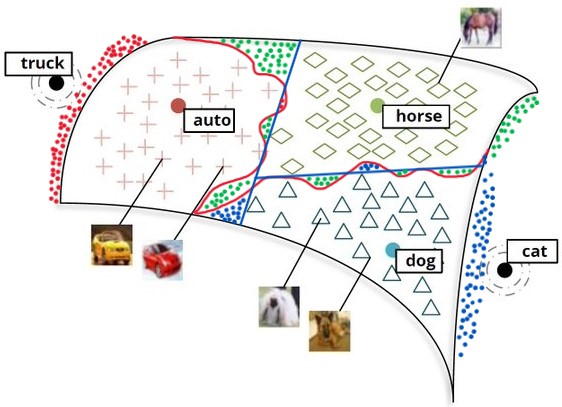
\includegraphics[width=1\textwidth, height=1\textheight, keepaspectratio]{manifold-hyp}
    \end{minipage}
    \begin{minipage}[c]{0.49\textwidth}
        \vspace{0pt}
        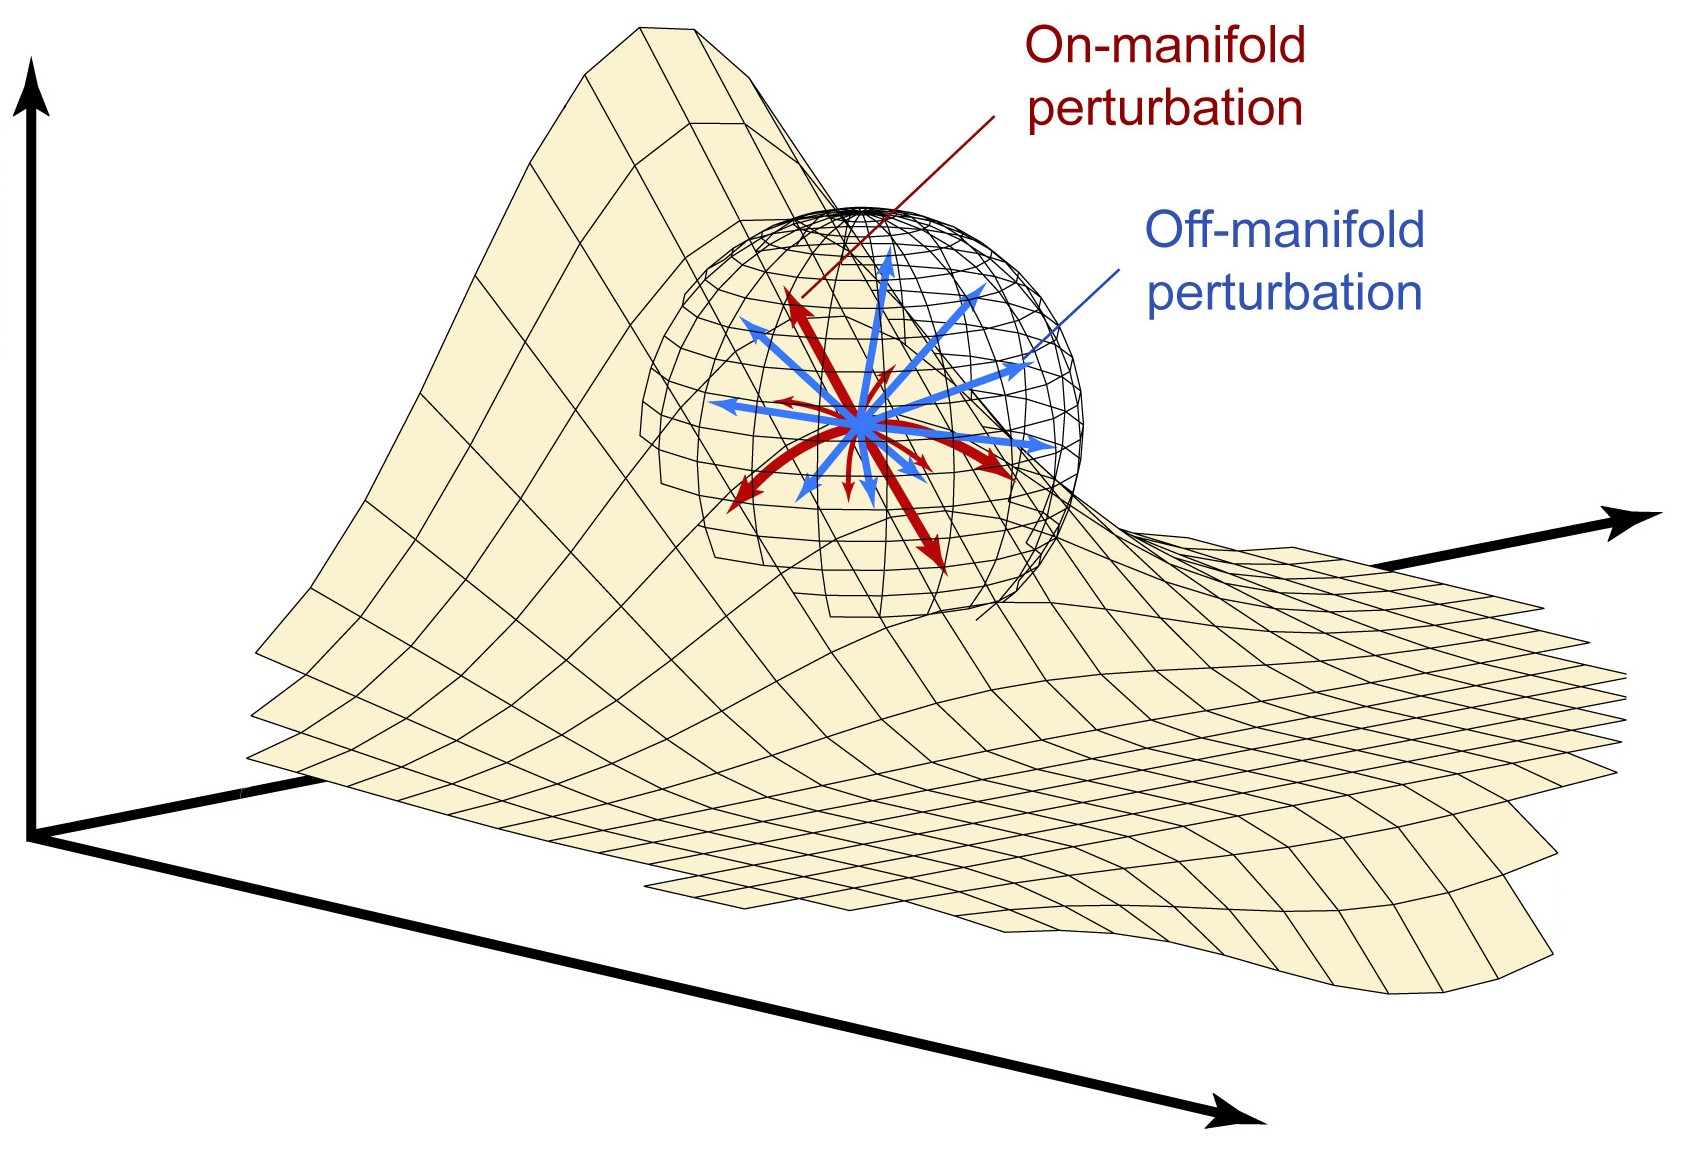
\includegraphics[width=1\textwidth, height=1\textheight, keepaspectratio]{manifold_ball_perturbations}
    \end{minipage}
    \hfill\break

    \texttt{CARSO} acts mainly as an \textit{on manifold re-projector}!

    \end{frame}

    \begin{frame}{\protect{\emoji{speaking-head}} Discussion (III)}

        \begin{block}{Time: a hidden cost?}
            Regardless of model performance, the \textit{training time} required for the \texttt{CARSO} portion of the alone is $\sim$ equivalent to that of \texttt{IAT} for the classifier. This results in a twofold increase in training time.

            Inference time sees a $\sim1500$-fold increase.
        \end{block}

    \underline{Note, however, that...}
    \begin{itemize}
        \item Overall training time is still (\textit{much}, even \textit{very much}; see \texttt{DefenseGAN} \textit{e.g.}) shorter than most \textit{better-than-\texttt{IAT}} approaches!
        \item \textit{W.r.t.} inference time, the method was originally targeted at \textit{high-stakes}, scenarios where such trade-off is acceptable. In case of realtime scenarios, also thanks to increased robustness, one can resort to \textit{stream thinning} (or \textit{fast-vs-slow} systems) if \texttt{CARSO} is deemed important.
    \end{itemize}
    \end{frame}

}

